% Options for packages loaded elsewhere
\PassOptionsToPackage{unicode}{hyperref}
\PassOptionsToPackage{hyphens}{url}
\PassOptionsToPackage{dvipsnames,svgnames*,x11names*}{xcolor}
%
\documentclass[
]{article}
\usepackage{lmodern}
\usepackage{amssymb,amsmath}
\usepackage{ifxetex,ifluatex}
\ifnum 0\ifxetex 1\fi\ifluatex 1\fi=0 % if pdftex
  \usepackage[T1]{fontenc}
  \usepackage[utf8]{inputenc}
  \usepackage{textcomp} % provide euro and other symbols
\else % if luatex or xetex
  \usepackage{unicode-math}
  \defaultfontfeatures{Scale=MatchLowercase}
  \defaultfontfeatures[\rmfamily]{Ligatures=TeX,Scale=1}
\fi
% Use upquote if available, for straight quotes in verbatim environments
\IfFileExists{upquote.sty}{\usepackage{upquote}}{}
\IfFileExists{microtype.sty}{% use microtype if available
  \usepackage[]{microtype}
  \UseMicrotypeSet[protrusion]{basicmath} % disable protrusion for tt fonts
}{}
\makeatletter
\@ifundefined{KOMAClassName}{% if non-KOMA class
  \IfFileExists{parskip.sty}{%
    \usepackage{parskip}
  }{% else
    \setlength{\parindent}{0pt}
    \setlength{\parskip}{6pt plus 2pt minus 1pt}}
}{% if KOMA class
  \KOMAoptions{parskip=half}}
\makeatother
\usepackage{xcolor}
\IfFileExists{xurl.sty}{\usepackage{xurl}}{} % add URL line breaks if available
\IfFileExists{bookmark.sty}{\usepackage{bookmark}}{\usepackage{hyperref}}
\hypersetup{
  pdftitle={Homework \#2},
  pdfauthor={Yunting Chiu},
  colorlinks=true,
  linkcolor=Maroon,
  filecolor=Maroon,
  citecolor=Blue,
  urlcolor=blue,
  pdfcreator={LaTeX via pandoc}}
\urlstyle{same} % disable monospaced font for URLs
\usepackage[margin=1in]{geometry}
\usepackage{color}
\usepackage{fancyvrb}
\newcommand{\VerbBar}{|}
\newcommand{\VERB}{\Verb[commandchars=\\\{\}]}
\DefineVerbatimEnvironment{Highlighting}{Verbatim}{commandchars=\\\{\}}
% Add ',fontsize=\small' for more characters per line
\usepackage{framed}
\definecolor{shadecolor}{RGB}{248,248,248}
\newenvironment{Shaded}{\begin{snugshade}}{\end{snugshade}}
\newcommand{\AlertTok}[1]{\textcolor[rgb]{0.94,0.16,0.16}{#1}}
\newcommand{\AnnotationTok}[1]{\textcolor[rgb]{0.56,0.35,0.01}{\textbf{\textit{#1}}}}
\newcommand{\AttributeTok}[1]{\textcolor[rgb]{0.77,0.63,0.00}{#1}}
\newcommand{\BaseNTok}[1]{\textcolor[rgb]{0.00,0.00,0.81}{#1}}
\newcommand{\BuiltInTok}[1]{#1}
\newcommand{\CharTok}[1]{\textcolor[rgb]{0.31,0.60,0.02}{#1}}
\newcommand{\CommentTok}[1]{\textcolor[rgb]{0.56,0.35,0.01}{\textit{#1}}}
\newcommand{\CommentVarTok}[1]{\textcolor[rgb]{0.56,0.35,0.01}{\textbf{\textit{#1}}}}
\newcommand{\ConstantTok}[1]{\textcolor[rgb]{0.00,0.00,0.00}{#1}}
\newcommand{\ControlFlowTok}[1]{\textcolor[rgb]{0.13,0.29,0.53}{\textbf{#1}}}
\newcommand{\DataTypeTok}[1]{\textcolor[rgb]{0.13,0.29,0.53}{#1}}
\newcommand{\DecValTok}[1]{\textcolor[rgb]{0.00,0.00,0.81}{#1}}
\newcommand{\DocumentationTok}[1]{\textcolor[rgb]{0.56,0.35,0.01}{\textbf{\textit{#1}}}}
\newcommand{\ErrorTok}[1]{\textcolor[rgb]{0.64,0.00,0.00}{\textbf{#1}}}
\newcommand{\ExtensionTok}[1]{#1}
\newcommand{\FloatTok}[1]{\textcolor[rgb]{0.00,0.00,0.81}{#1}}
\newcommand{\FunctionTok}[1]{\textcolor[rgb]{0.00,0.00,0.00}{#1}}
\newcommand{\ImportTok}[1]{#1}
\newcommand{\InformationTok}[1]{\textcolor[rgb]{0.56,0.35,0.01}{\textbf{\textit{#1}}}}
\newcommand{\KeywordTok}[1]{\textcolor[rgb]{0.13,0.29,0.53}{\textbf{#1}}}
\newcommand{\NormalTok}[1]{#1}
\newcommand{\OperatorTok}[1]{\textcolor[rgb]{0.81,0.36,0.00}{\textbf{#1}}}
\newcommand{\OtherTok}[1]{\textcolor[rgb]{0.56,0.35,0.01}{#1}}
\newcommand{\PreprocessorTok}[1]{\textcolor[rgb]{0.56,0.35,0.01}{\textit{#1}}}
\newcommand{\RegionMarkerTok}[1]{#1}
\newcommand{\SpecialCharTok}[1]{\textcolor[rgb]{0.00,0.00,0.00}{#1}}
\newcommand{\SpecialStringTok}[1]{\textcolor[rgb]{0.31,0.60,0.02}{#1}}
\newcommand{\StringTok}[1]{\textcolor[rgb]{0.31,0.60,0.02}{#1}}
\newcommand{\VariableTok}[1]{\textcolor[rgb]{0.00,0.00,0.00}{#1}}
\newcommand{\VerbatimStringTok}[1]{\textcolor[rgb]{0.31,0.60,0.02}{#1}}
\newcommand{\WarningTok}[1]{\textcolor[rgb]{0.56,0.35,0.01}{\textbf{\textit{#1}}}}
\usepackage{graphicx,grffile}
\makeatletter
\def\maxwidth{\ifdim\Gin@nat@width>\linewidth\linewidth\else\Gin@nat@width\fi}
\def\maxheight{\ifdim\Gin@nat@height>\textheight\textheight\else\Gin@nat@height\fi}
\makeatother
% Scale images if necessary, so that they will not overflow the page
% margins by default, and it is still possible to overwrite the defaults
% using explicit options in \includegraphics[width, height, ...]{}
\setkeys{Gin}{width=\maxwidth,height=\maxheight,keepaspectratio}
% Set default figure placement to htbp
\makeatletter
\def\fps@figure{htbp}
\makeatother
\setlength{\emergencystretch}{3em} % prevent overfull lines
\providecommand{\tightlist}{%
  \setlength{\itemsep}{0pt}\setlength{\parskip}{0pt}}
\setcounter{secnumdepth}{-\maxdimen} % remove section numbering

\title{Homework \#2}
\author{Yunting Chiu}
\date{2021-02-01}

\begin{document}
\maketitle

\begin{enumerate}
\def\labelenumi{\arabic{enumi}.}
\tightlist
\item
  (\textbf{1.2}) The members of a health spa pay annual membership dues
  of \$\$\$300 plus a charge of \$\$\$2 for each visit to the spa. Let Y
  denote the dollar cost for the year for a member and X the number of
  visits by the member during the year. Express the relation between X
  and Y mathematically. Is it a functional relation or a statistical
  relation (that is, is the relation deterministic or stochastic)?
\end{enumerate}

\begin{itemize}
\tightlist
\item
  deterministic: the output of the model is entirely determined by the
  values of the parameters and the initial conditions; stochastic:
  random, unpredictable.
\item
  The association between X and Y is: Y = 300 + 2X (dollars).\\
  This is a functional relationship because a effect in the value of the
  X will cause the corresponding change in the value of the Y. X and Y
  will not have a uncertain effect.
\end{itemize}

\begin{enumerate}
\def\labelenumi{\arabic{enumi}.}
\setcounter{enumi}{1}
\tightlist
\item
  (\textbf{1.6}) Suppose the regression parameters are \(\beta0\) = 200
  and \(\beta1\) = 5.0.\\
\end{enumerate}

\begin{enumerate}
\def\labelenumi{(\alph{enumi})}
\tightlist
\item
  Plot the regression equation.\\
\end{enumerate}

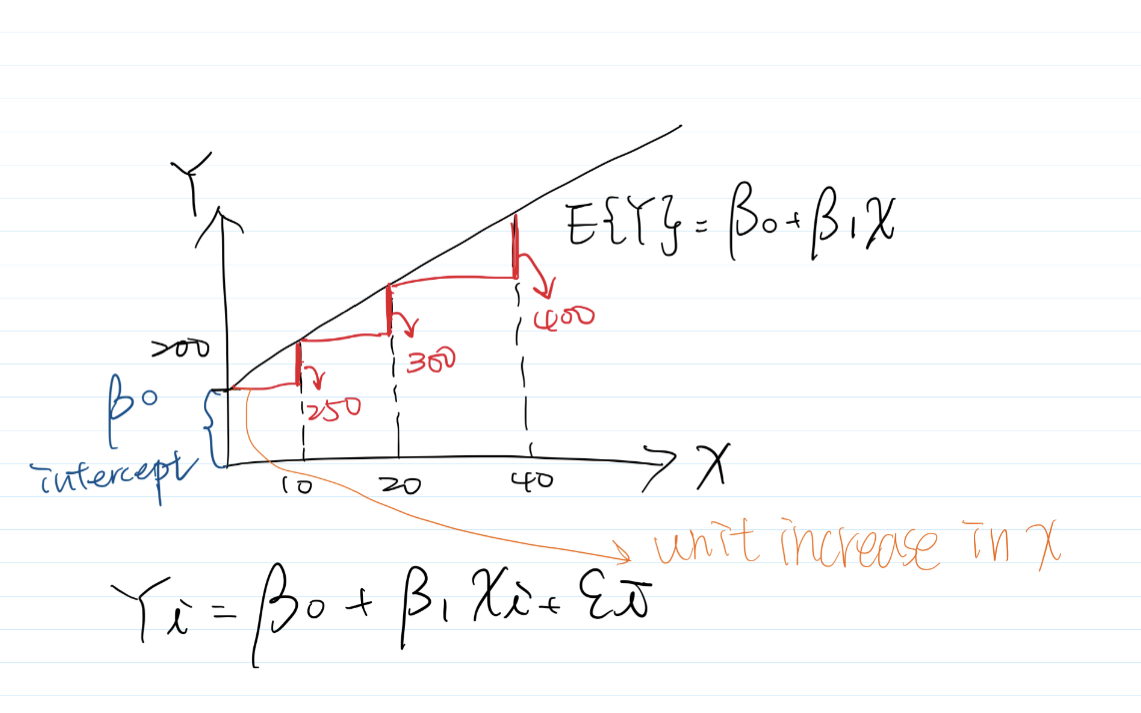
\includegraphics{pics/IMG_445592DDC4E5-1.jpeg}

\begin{enumerate}
\def\labelenumi{(\alph{enumi})}
\setcounter{enumi}{1}
\tightlist
\item
  Predict the response for X = 10, 20, and 40.\\
\end{enumerate}

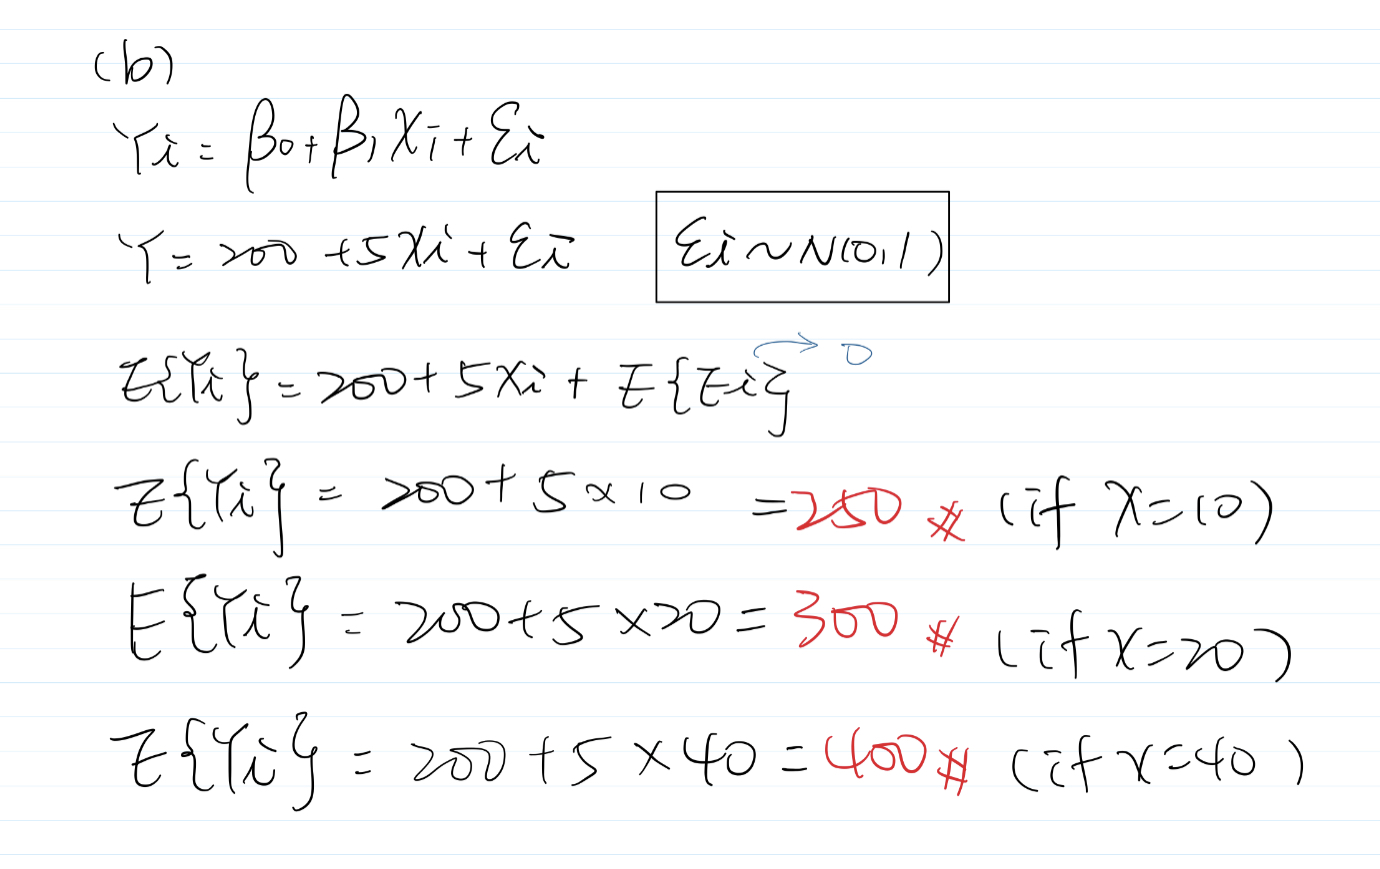
\includegraphics{pics/IMG_BEAC2260AB98-1.jpeg}

\begin{enumerate}
\def\labelenumi{(\alph{enumi})}
\setcounter{enumi}{2}
\tightlist
\item
  Explain the meaning of parameters \(\beta0\) and \(\beta1\).\\
\end{enumerate}

\begin{itemize}
\tightlist
\item
  \(\beta0\) = Y intercept of regression line.
\item
  \(\beta1\): one unit change in X, generates a \(\beta1\) unit change
  in Y.
\end{itemize}

\begin{enumerate}
\def\labelenumi{\arabic{enumi}.}
\setcounter{enumi}{2}
\tightlist
\item
  (\textbf{1.10}) An analyst in a large corporation studied the relation
  between current annual salary (Y ) and age (X) for the 46 computer
  programmers presently employed in the company. The analyst concluded
  that the relation is curvilinear, reaching a maximum at 47 years. Does
  this imply that the salary for a programmer increases until age 47 and
  then decreases? Explain.
\end{enumerate}

\begin{itemize}
\tightlist
\item
  \textbf{curvilinear} only explain that X and Y are not linear
  relation. It is not true because it reaches its maximum at a point and
  then increasing at a decreasing rate meaning that wage first increases
  to a max at year 47 and then the increasing rate slows down. In
  reality, decreasing salary as people age in any company is not make
  sense, we also can find a bunch of examples in real world.
\end{itemize}

\begin{enumerate}
\def\labelenumi{\arabic{enumi}.}
\setcounter{enumi}{3}
\tightlist
\item
  The time it takes to transmit a file always depends on the file size.
  Suppose you transmitted 30 files, with the average size of 126 Kbytes
  and the standard deviation of 35 Kbytes. The average transmittance
  time was 0.04 seconds with the standard deviation of 0.01 seconds. The
  correlation coefficient between the time and the size was 0.86. Based
  on this data, fit a linear regression model and predict the time it
  will take to transmit a 400 Kbyte file.
\end{enumerate}

\begin{itemize}
\tightlist
\item
  Based on the model above, it will take 0.1085 sec to transmit a 400
  Kbyte file.
\end{itemize}

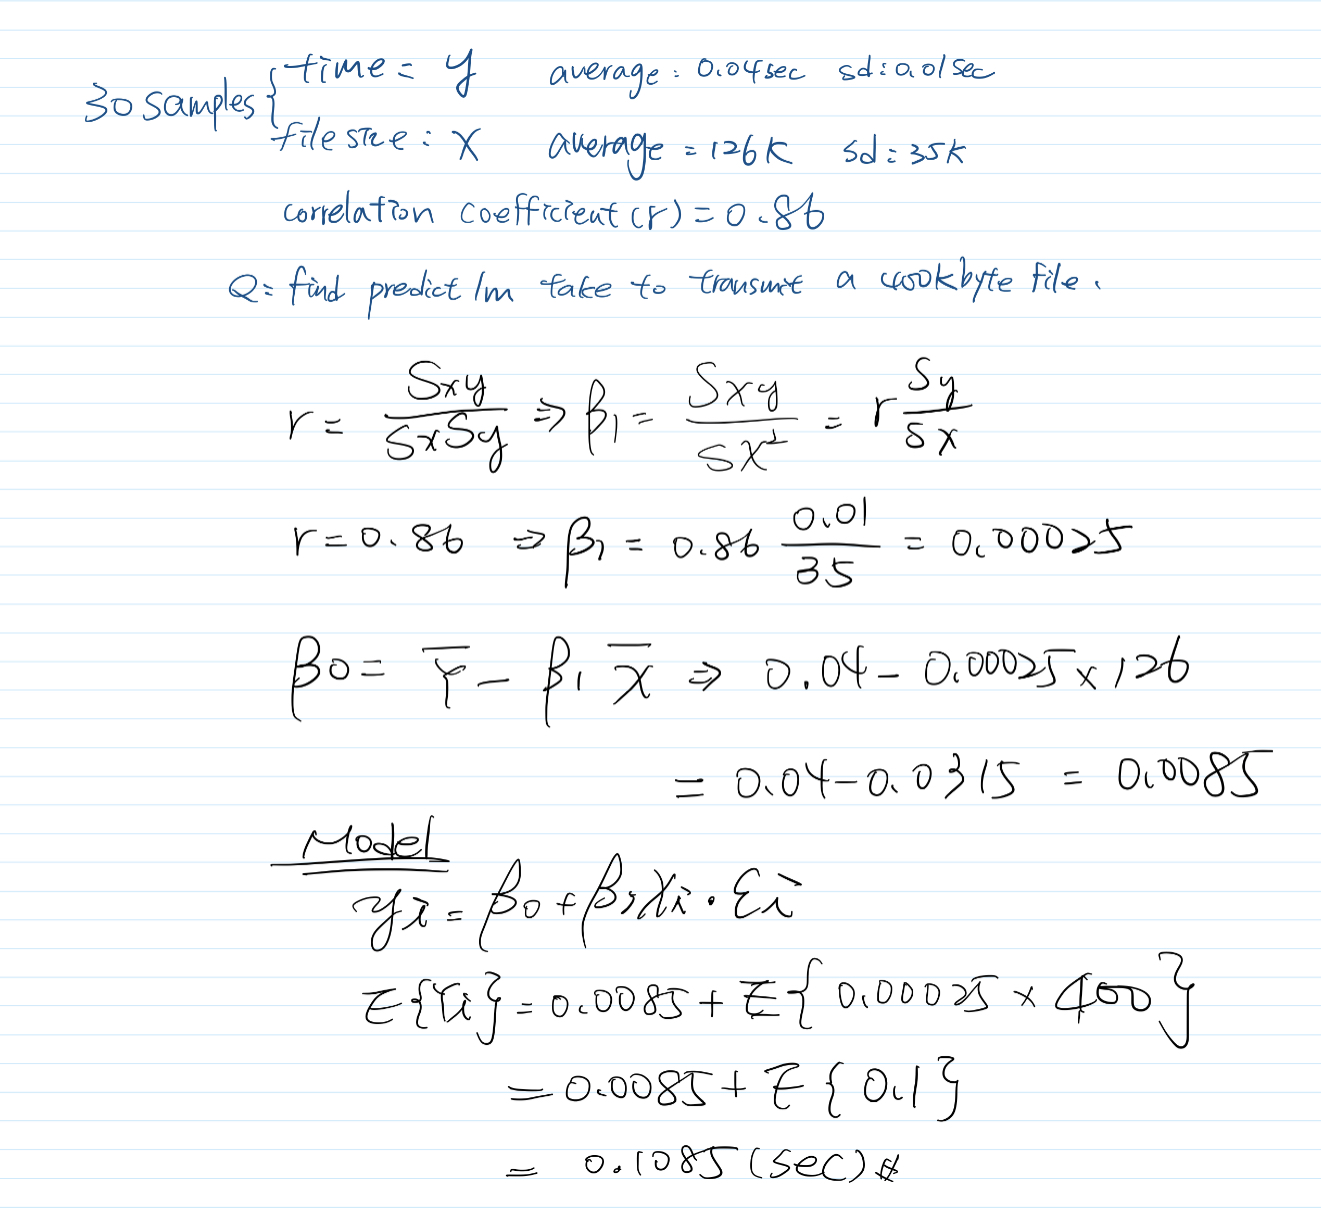
\includegraphics{pics/IMG_0445139B99EC-1.jpeg}

\begin{enumerate}
\def\labelenumi{\arabic{enumi}.}
\setcounter{enumi}{4}
\tightlist
\item
  At a gas station, 180 drivers were asked to record the mileage of
  their cars and the number of miles per gallon. The results are
  summarized in the table.\\
\end{enumerate}

\begin{enumerate}
\def\labelenumi{(\alph{enumi})}
\tightlist
\item
  Compute the least squares regression line which describes how the
  number of miles per gallon depends on the mileage.\\
\item
  What do the obtained slope and intercept mean in this situation?\\
\item
  You purchase a used car with 35,000 miles on it. Predict the number of
  miles per gallon.\\
\end{enumerate}

\begin{enumerate}
\def\labelenumi{\arabic{enumi}.}
\setcounter{enumi}{5}
\item
  (Stat-615 only) Show that the sample intercept b0 is a linear and
  unbiased estimator of the population intercept \(\beta0\).
\item
  (Computer project - 1.19, 1.24). Grade point average. The director of
  admissions of a small college selected 120 students at random from the
  new freshman class in a study to determine whether a students grade
  point average (GPA) at the end of the freshman year (Y) can be
  predicted from the ACT test score (X). The results of the study
  follow.\\
\end{enumerate}

\begin{enumerate}
\def\labelenumi{(\alph{enumi})}
\tightlist
\item
  Obtain the least squares estimates of β0 and β1 and state the
  estimated regression function.\\
\item
  Plot the estimated regression function and the data. Does the
  estimated regression function appear to fit the data well?\\
\item
  Obtain a point estimate of the mean freshman GPA for students with ACT
  test score X = 30.\\
\item
  What is the point estimate of the change in the mean response when the
  entrance test score increases by one point?\\
\item
  Obtain the residuals ei and the sum of the squared residuals 􏰀 e2i .\\
\item
  Obtain point estimates of σ2 and σ. In what units is each of them
  expressed?\\
\end{enumerate}

\begin{Shaded}
\begin{Highlighting}[]
\KeywordTok{library}\NormalTok{(tidyverse)}
\end{Highlighting}
\end{Shaded}

\begin{verbatim}
## -- Attaching packages --- tidyverse 1.3.0 --
\end{verbatim}

\begin{verbatim}
## v ggplot2 3.3.2     v purrr   0.3.4
## v tibble  3.0.3     v dplyr   1.0.2
## v tidyr   1.1.2     v stringr 1.4.0
## v readr   1.3.1     v forcats 0.5.0
\end{verbatim}

\begin{verbatim}
## -- Conflicts ------ tidyverse_conflicts() --
## x dplyr::filter() masks stats::filter()
## x dplyr::lag()    masks stats::lag()
\end{verbatim}

\begin{Shaded}
\begin{Highlighting}[]
\NormalTok{aaa <-}\StringTok{ }\KeywordTok{read_tsv}\NormalTok{(}\StringTok{"./data/CH01PR19.txt"}\NormalTok{)}
\end{Highlighting}
\end{Shaded}

\begin{verbatim}
## Parsed with column specification:
## cols(
##   `3.897    21` = col_character()
## )
\end{verbatim}

\begin{Shaded}
\begin{Highlighting}[]
\NormalTok{aaa}
\end{Highlighting}
\end{Shaded}

\begin{verbatim}
## # A tibble: 119 x 1
##    `3.897    21`
##    <chr>        
##  1 3.885    14  
##  2 3.778    28  
##  3 2.540    22  
##  4 3.028    21  
##  5 3.865    31  
##  6 2.962    32  
##  7 3.961    27  
##  8 0.500    29  
##  9 3.178    26  
## 10 3.310    24  
## # ... with 109 more rows
\end{verbatim}

\end{document}
